\subsection{TET Histograms and Distance}\label{Subsec:TET_historgram_and_distance}
	A method that can be used to find similarity between the TETs is to transform the TETs into histograms and compare these\cite{JAEGER201330}.
	\begin{figure}[H]
		\centering
		\begin{adjustbox}{width=0.5\textwidth}
			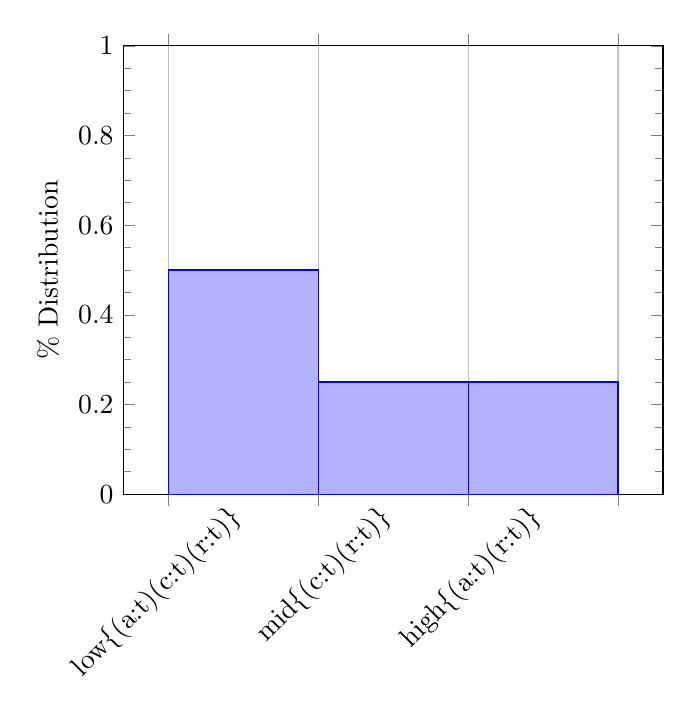
\begin{tikzpicture}
	\begin{axis}[
	ybar interval, 
	ymax=1,ymin=0, 
	minor y tick num = 3,
	ylabel = {\% Distribution},
	symbolic x coords={low\{(a:t)(c:t)(r:t)\}, mid\{(c:t)(r:t)\}, high\{(a:t)(r:t)\}, high\{(y:t)(r:t)\}},
	x tick label style={font=\normalsize, rotate=45, anchor=east},
	]
	\addplot coordinates {(low\{(a:t)(c:t)(r:t)\}, 0.5) (mid\{(c:t)(r:t)\}, 0.25) (high\{(a:t)(r:t)\}, 0.25) (high\{(y:t)(r:t)\}, 0.10)};
	\end{axis}
\end{tikzpicture}

%\begin{tikzpicture}

%\definecolor{bblue}{HTML}{4F81BD}

%\begin{axis}[
%major x tick style = transparent,
%ymin=0,
%bar width=1cm,
%minor y tick num = 3,
%ymajorgrids = true,
%ylabel = {\% distribution},
%symbolic x coords={low\{(a:t)(c:t)(r:t)\}, mid\{(c:t)(r:t)\}, high\{(a:t)(r:t)\}},
%xtick = data,
%x tick label style={font=\normalsize, rotate=45, anchor=east},
%]
%\addplot[ybar , style={bblue,fill=bblue,mark=none}]
%coordinates {(low\{(a:t)(c:t)(r:t)\}, 0.5) (mid\{(c:t)(r:t)\}, 0.25) (high\{(a:t)(r:t)\}, 0.25)};

%\end{axis}
%\end{tikzpicture}
		\end{adjustbox}
		\caption{The TET histogram derived from \autoref{fig:Tet_example}}
		\label{fig:Tethistogram}
	\end{figure}

	By comparing the key for each node in each level of the tree, we can find the structural difference. For example if comparing two TETs we know that if the users in the TETs are equal, then we work on the same tree and the distance is $0$. Considering the rating level for \autoref{fig:Tet_example} we define the equivalent histogram in \autoref{fig:Tethistogram}. On this level, we compare low, medium and high by assigning them a numeric value.

	On the genre level of the TET we find the different child nodes for each node in the earlier histogram \autoref{fig:Tethistogram}. As an example for  \autoref{fig:Tethistogram} we have the node  $low\{(a:t)(c:t)(r:t)\}$. This node will be split for each genre,  and the child nodes will then be  $(a:t)$, $(c:t)$ and $(r:t)$. We can use manhatten distance at this level by considering it as a vector. Here, comparison with another histogram with less \textit{true} genre features than the other can then be compared as seen in \autoref{Eq:manhattencomparason}\cite{singh2013k}.

	When comparing two histograms, one histogram might have some elements that the other does not have. For any missing element in a histogram we add the value $0$, and we are thereby able to calculate distance for the missing element.

	\begin{equation}\label{Eq:manhattencomparason}
	D(\begin{bmatrix}
	x_{1.1} \\
	x_{1.2} \\
	x_{1.3}
	\end{bmatrix},
	\begin{bmatrix}
	x_{2.1} \\
	x_{2.2}
	\end{bmatrix})= |x_{1.1} - x_{2.1}| + |x_{1.2} - x_{2.2}| + |x_{1.3} - 0|
	\end{equation}

	The general formula for these comparisons can be seen in \autoref{Eq:manhattencomparason} and \autoref{eq:compare_tet}
	\begin{equation}\label{eq:compare_tet}
	\begin{split}
	D(h,h') = \sum_{i=1}^{max(|h|,|h'|)} & (D(h^{\downarrow}, h'^{\downarrow})+ D(h_{key}, h'_{key}))  \\
	& * distribution(h) * distribution (h')
	\end{split}
	\end{equation}

	In \autoref{eq:compare_tet} $h^{\downarrow}$ means the TETs next level histogram representation. The $distribution()$ adds the importance for each of the type of subTETs.
